\lfoot{Autor: Raphael Simek}
\subsubsection{Motorwirkungsgrad}
\label{subsec:motorwirkungsgrad}

\textbf{Einführung\newline}
Grundsätzlich beschäftigten wie uns mit dem Motorwirkungsgrad, um feststellen zu können, welcher Schaltpunkt möglichst effizient bezüglich des Motorwirkungsgrads ist. Denn es gibt unterschiedliche Wirkungsgrade, deshalb heißt ein niedriger Spritverbrauch (Motorwirkungsgrad) nicht gleichzeitig ein niedriger \ce{CO2}-Ausstoß. Der Katalysator hat also einen eigenen Wirkungsgrad, welcher für diese Rechnung einbezogen werden muss. Für das Diplomprojekt beschlossen wir den Motorwirkungsgrad in den Fokus zu setzen.

\textbf{\newline Heutige Probleme durch die Öl-Förderung}
\begin{wrapfigure}{r}{0.6\textwidth}\centering
    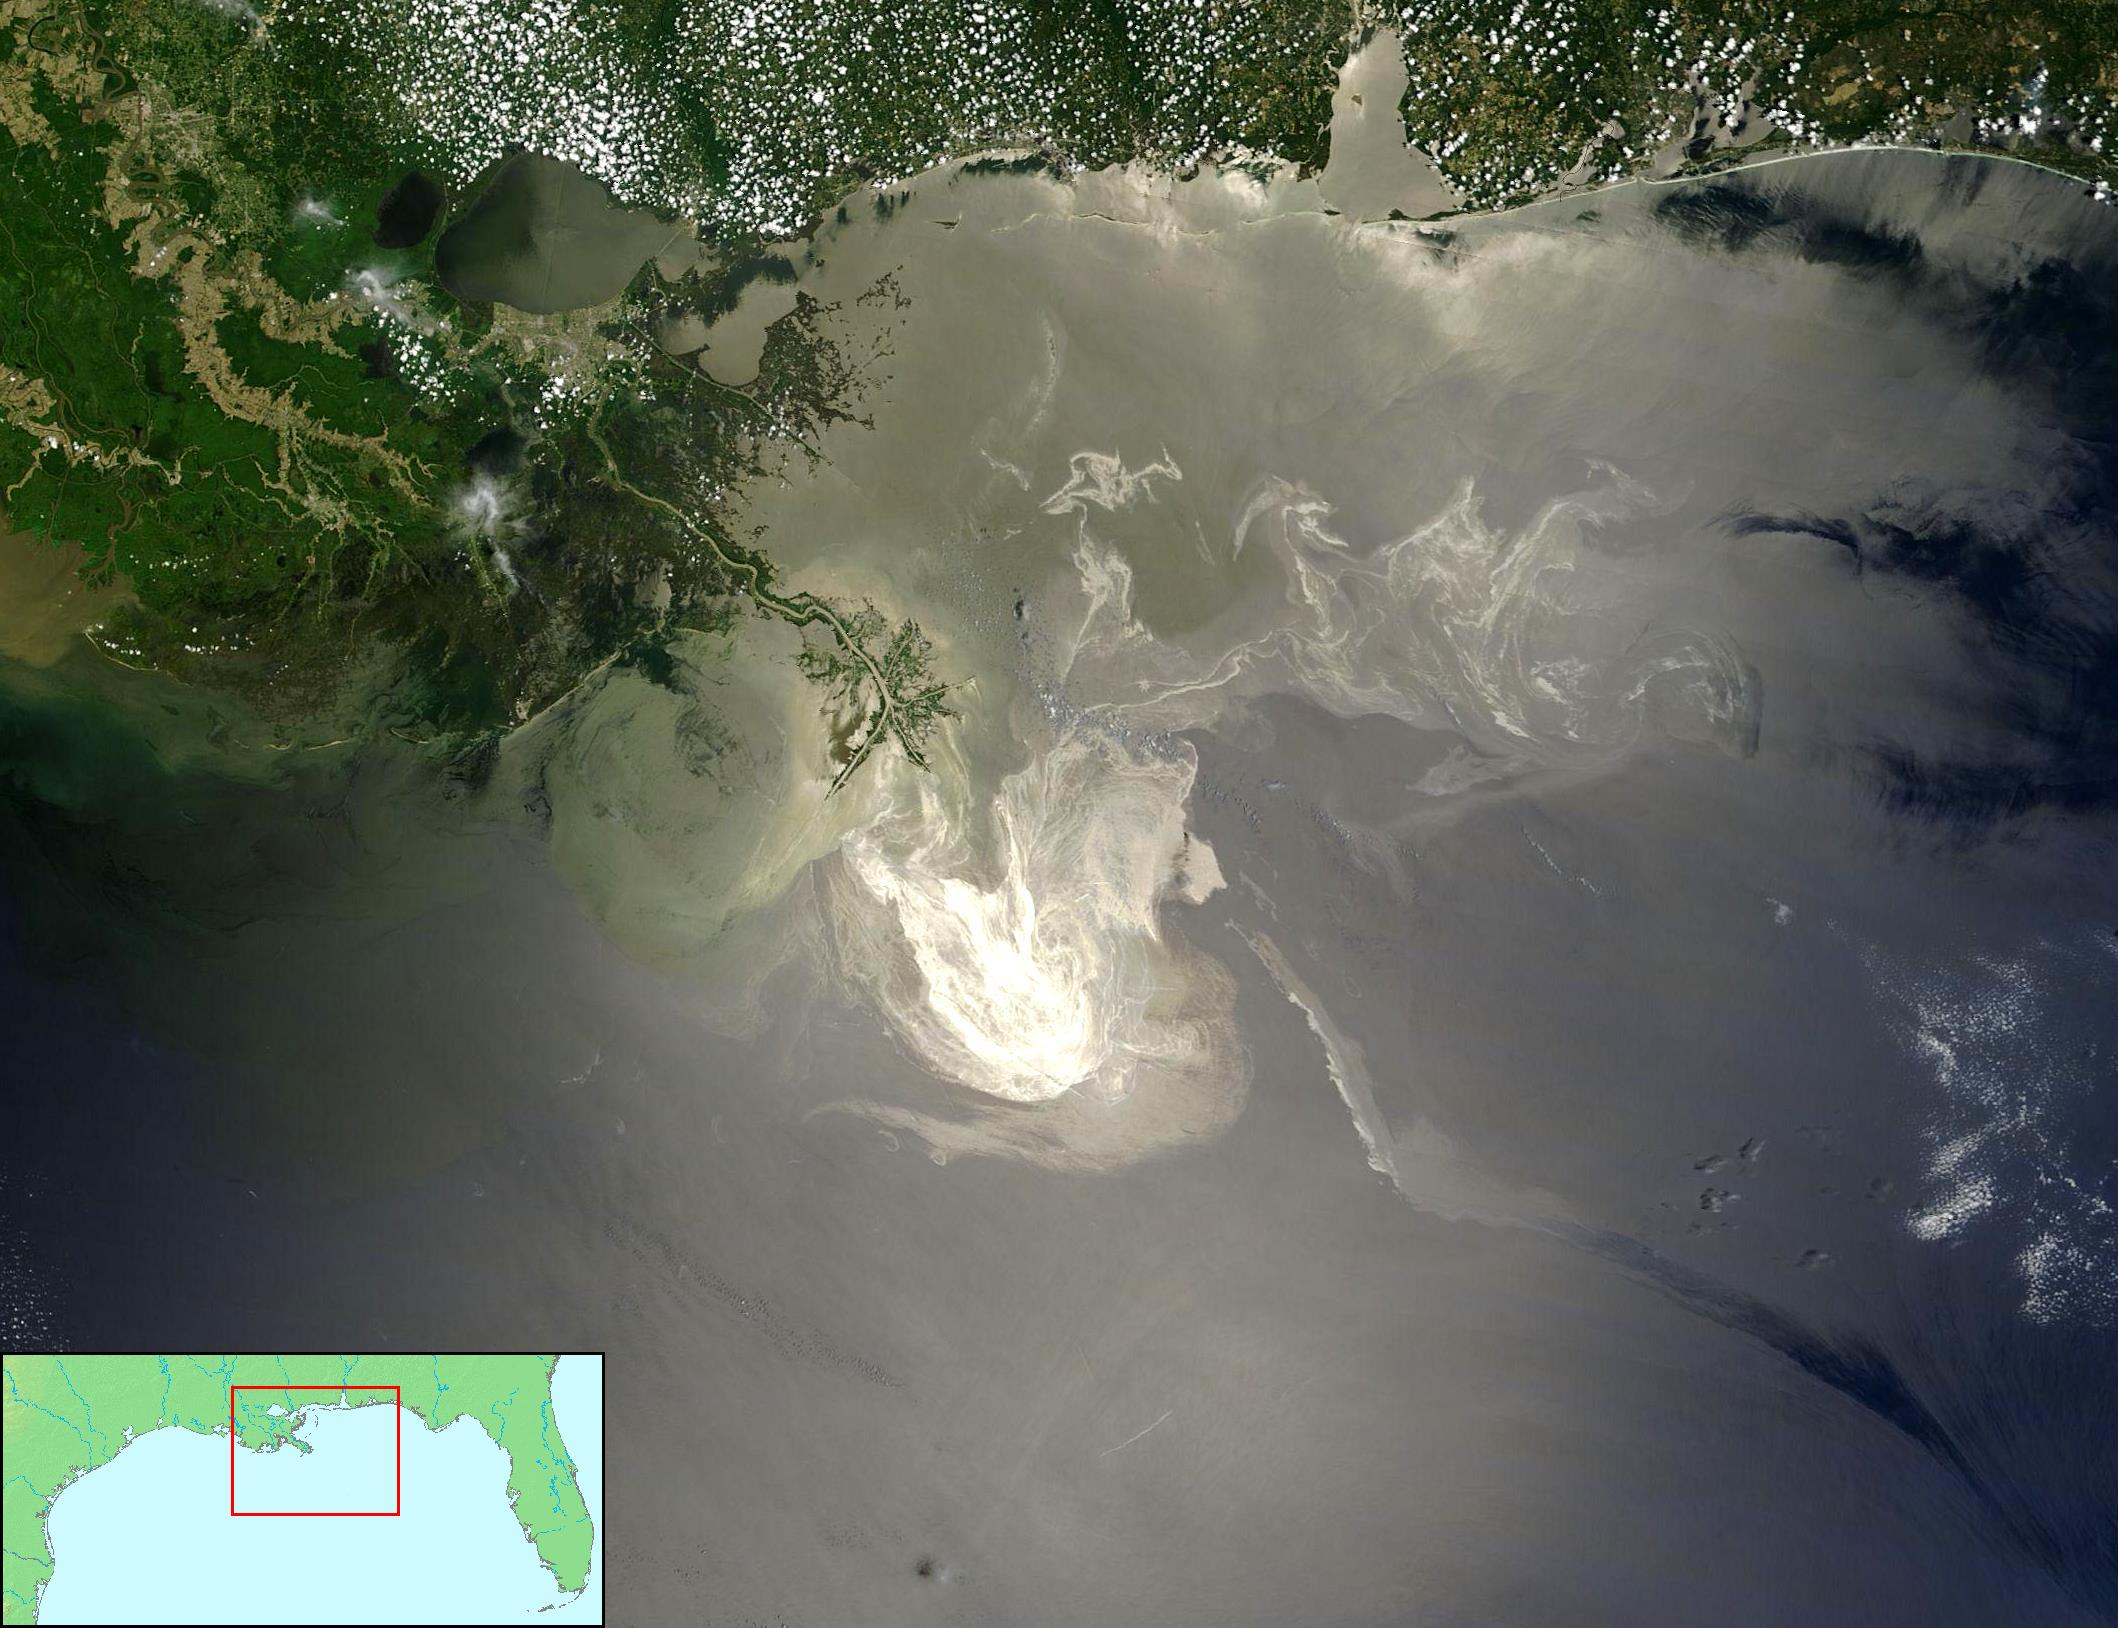
\includegraphics[width=0.6\textwidth]{images/bpOilSpillSatelite}
    \caption{1 Monat nach der Explosion \cite{SIMR.CH2-motorwirkungsgrad.bpOilSpillSatelite}} \label{Fig:imgBPOilSpill}
\end{wrapfigure}
Dieses Thema ist besonders in Bezug auf die immer restriktiveren Emissionsbestimmungen und die häufig hohen Kraftstoffpreise von Interesse für Autofahrer. Zusätzlich sind fossile Brennstoffe, bekanntlich, nicht erneuerbare Ressourcen, weshalb die Vorkommen zeitnah erschöpft sein werden. Genau deshalb ist es besonders wichtig sparsam und ökonomisch mit der bald erschöpften Ressource Erdöl umzugehen. 
Denn die Öl-Förderung erzeugt schon heute Naturkatastrophen und Umweltverschmutzung und wird immer schwerer zu erlangen.
Naturkatastrophen wie BP's \textit{Deepwater Horizon} Ölpest aus dem Jahre 2010 \cite{SIMR.CH2-motorwirkungsgrad.BPSpillGeneral}, bei welcher 3 Jahre nach der Explosion weiterhin Rekordzahlen von Delphinen und Wasserschildkröten starben \cite{SIMR.CH2-motorwirkungsgrad.BPSpillDeaths}. 

Die Probleme, die durch die Öl-Förderung entstehen enden aber noch nicht hier, denn Öl wird auch immer schwerer zu erreichen. Deshalb müssen Techniken wie Fracking eingesetzt werden, um die letzen Öl-Reserven zwischen den Bohrungen zu fördern, wofür ein Cocktail von für Menschen giftigen und sogar radioaktiven Chemikalien verwendet werden \cite{SIMR.CH2-motorwirkungsgrad.FrackingChemicals}. Es wird geschätzt dass 30-70\% dieses Cocktails wieder an die Oberfläche kommen wird und das Grundwasser verseuchen wird \cite{SIMR.CH2-motorwirkungsgrad.FrackingGroundwater}.

\begin{figure}[!htb]\centering
	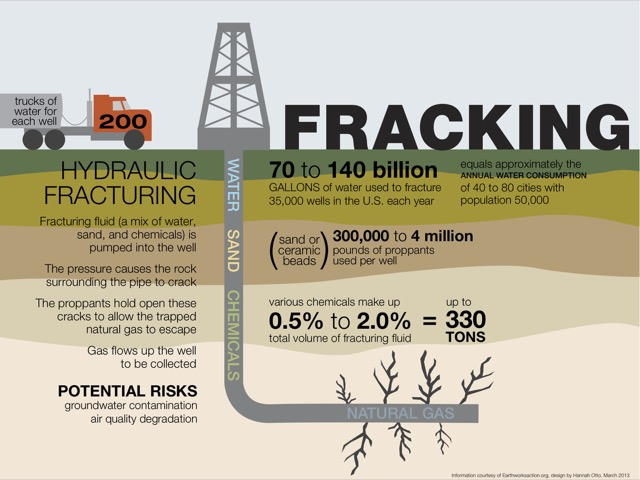
\includegraphics[width=0.6\textwidth]{images/frackingInfographic}
	\caption{Fracking in einem Bild erklärt \cite{SIMR.CH2-motorwirkungsgrad.frackingDescription}}\label{Fig:imgFrackingDesc}
\end{figure}

\newpage
\textbf{zukünftige Probleme durch Öl-Förderung\nextline}
All diese, bereits vorkommenden, Probleme scheinen aber in keinem Verhältnis zu den Problemen die uns erwarten, wenn wir alles Öl auf der Erde verbrauchen, zu stehen. Sollten wir nämlich alles Öl auf der Erde verbrennen, so würde uns ein Anstieg des Ozeans um 44ft (13.41m) erwarten. \cite{SIMR.CH2-motorwirkungsgrad.SeaLevelRiseAllOilBurnt} Da dies aber unwahrscheinlich zeitnah passieren wird, wurde auch ein Anstieg von 4ft (0.91m) innerhalb eines Jahrhunderts, bei anhaltendem Ölverbrauch, von der NASA vorhergesagt. \cite{SIMR.CH2-motorwirkungsgrad.SeaLevelRiseCentury}

\begin{figure}[!htb]\centering
	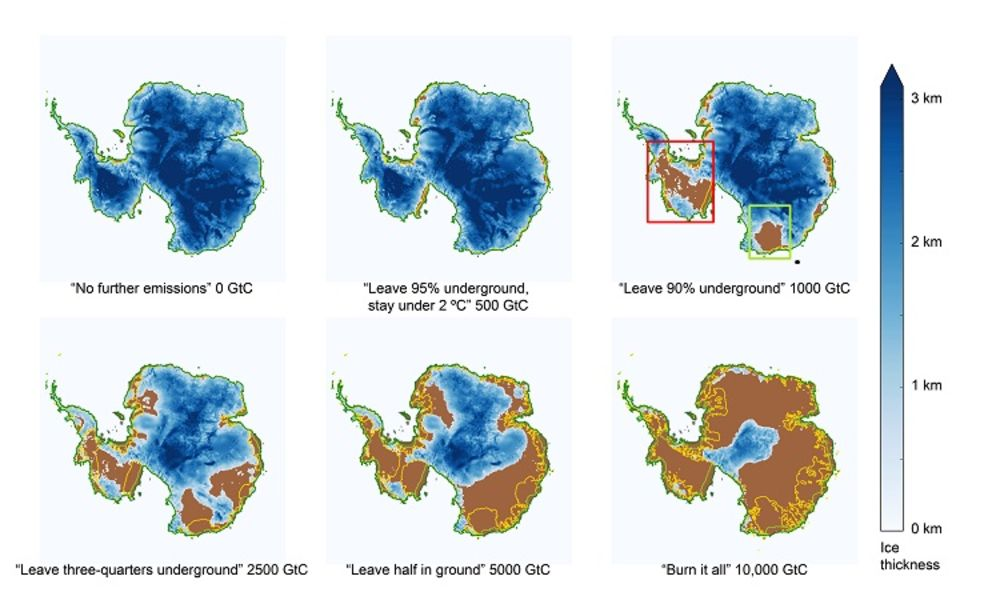
\includegraphics[width=0.8\textwidth]{images/greenlandSeaLevel}
	\caption{Grafik die die Polarschmelzung, nach Ölmenge, illustriert \cite{SIMR.CH2-motorwirkungsgrad.SeaLevelRiseAllOilBurnt}}\label{Fig:imgGreenlandMelting}
\end{figure}

\newpage
\textbf{Zielsetzung\newline}
Gewollt war also ein möglichst kraftstoffeffizienter Schaltvorschlag, doch um verstehen zu können wieso der Schaltvorschlag funktioniert, ist zuerst einiges an Grundwissen nötig.
Jeder der ein Auto fährt kennt diese Formel \textit{Kraftstoffmenge = Strecke * Verbrauch}. So kann man also entweder weniger fahren oder verbrauchsärmer fahren. Wir möchten uns hier auf 2. konzentrieren. Nur konsequent verfolgte Tipps lassen eine echte Veränderung im Verbrauch erkennen, auch das ist einem Großteil der Autofahrer bekannt, doch welche Tipps lohnt es sich anzuwenden? Dazu später mehr, zuerst mehr zu den momentanen Autos und deren physikalische Hintergründe.
Einigen von Ihnen sind Wahrscheinlich die Prozesse hinter einem 4-Takt Motor ein Begriff, trotzdem möchte ich diese hier kurz zusammenfassen und besonders auf die Energieverluste bei diesem Prozess eingehen:

\begin{figure}[!htb]\centering
	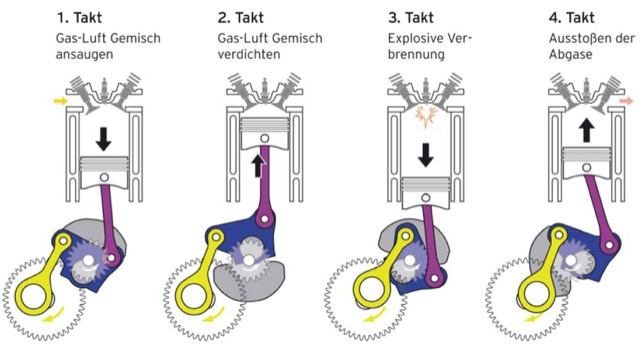
\includegraphics[width=0.8\textwidth]{images/viertaktMotorPrinzip}
	\caption{Prinzip eines 4-Takt Motors \cite{SIMR.CH2-motorwirkungsgrad.4strokeEngine}}\label{Fig:img4strokeEngine}
\end{figure}

Verlorene Energie bei der Verbrennung:
\textit{direktes Zitat: \cite{SIMR.CH1-Fahrstil-Analyse.Motorkennfeld}}
\begin{itemize}
	\item Auspuff: 36\% ausgestoßene Wärme
	\item Durch Zylinderwände: 33\% Abwärme, Teil davon für die Heizung
	\item Motorreibung: Reibung verlangt der Motorbewegung 8\% der Gesamtenergie ab
\end{itemize}
So bleiben im besten Falle 25\% über, die auf die Reifen übertragen werden. Diese 25\% sind zumeist nur unter Volllast erreichbar. Neue TDI Diesel-Motoren schaffen im Optimalfall einen Wirkungsgrad von 30\%, das ist aber bei Verbrennungsmotoren das Optimum. Wenn man nun aber Verbrauchsschonend fährt, so erreicht man meist nur einen Wirkungsgrad von 10\%. Diese wenige Energie die der Motor, aus dem Tropfen Kraftstoff, der eingespritzt wird, erlangt, wird dann durch folgende Widerstände erneut geschwächt:
\textit{direktes Zitat: \cite{SIMR.CH1-Fahrstil-Analyse.Motorkennfeld}}
\begin{itemize}
	\item Beschleunigungswiderstand: Das Beschleunigen eines Körpers braucht Energie. Die Energie wächst quadratisch mit der Geschwindigkeit, sie bleibt aber als \textit{kinetische Energie} in der Geschwindigkeit. 
	\item Steigungswiderstand: Nutzenergie wird beim Bergauffahren gebraucht. Sie bleibt als \textit{potenzielle Energie} gespeichert, welche Abgerufen wird, wenn wieder bergab gefahren wird.
	\item Rollreibung: Diese stellt sich jeder Bewegung in den Weg. Je nach Beschaffenheit der Straße und der Reifen reiben beide aneinander und erwärmen sich. Bei steigender Geschwindigkeit oder niedrigem Reifendruck steigt diese Reibung an.
	\item Luftwiderstand: Diese verdrückt mit zunehmender Geschwindigkeit mehr Energie. Weil bei doppelter Geschwindigkeit nicht nur doppelt so viel Luft verdrängt werden muss, sondern sie auch mit doppelter Geschwindigkeit aufprallt, wächst die bremsende Kraft quadratisch. 
	\item (Bremsen): Dieser Widerstand tritt nicht ständig auf, sondern hängt ausschließlich von seinem Fahrstil ab. Hierbei ist der häufige Wechsel von beschleunigen und bremsen gemeint, was so erneut einen quadratischen Widerstand darstellt. 
\end{itemize}

Alle diese Faktoren sind zumeist von Ihrem eigenen Fahrstil abhängig, welcher dadurch auch Ihren Verbrauch diktiert. Daraus folgt also dass versucht werden muss diese Widerstände durch möglichst effektives Fahren im Straßenverkehr so gering als möglich zu halten.

\textbf{Motorwirkungsgrad\nextline}
Die Zielsetzung des Projektes ist es das Fahrzeug in möglichst hohem Motorwirkungsgrad zu halten, das heißt dass aus jedem Tropfen eingespritztem Kraftstoff möglichst viel Energie gewonnen werden soll. Deshalb wird bei diesem Ansatz auch bewusst dazu aufgefordert den Motor weitaus höher als bei einem konventionellen Schaltvorschlag zu drehen bzw. mit höherer Motorlast zu fahren.
 
Viele Autos bieten im Gegensatz dazu zum Zweck der Verbrauchsmessung nur eine Anzeige des Momentanverbrauchs, welcher wenig hilfreich ist, denn mit dieser Berechnung kann man keine Schlüsse auf die Fahrweise ziehen. Außerdem unterscheiden sich Bordcomputer von einander oft stark. Einige Glätten den Verbrauch auf einen Zeitraum, einige lügen hohe Verbräuche weg, doch alle gemeinsam haben sie, dass die nicht ausreichend dokumentiert sind um faktische Rückschlüsse auf den Fahrstil treffen zu können.

Das ließe sich durch ein einheitliches System aus Hardware und Software vereinheitlichen, wodurch man dann vergleichbare Einheiten, die bei jedem Fahrzeug gleich sind erhalten würde. 

\textbf{Bonanza-Effekt oder Torsionsschwingungen im Antriebsstrang\nextline}
Direktes Zitat: \cite{SIMR.CH2-motorwirkungsgrad.Motorschwingungen}
\textit{
\"Der Verkehr stockt und zwingt den Autofahrer zum Bremsen, er schaltet jedoch nicht in einen niedrigeren Gang. In solchen Fällen ist oftmals ein Brummen zu hören: Die Torsionsschwingung verursacht das unangenehme Geräusch. Sie tritt auf, da sich die Kurbelwelle bei Verbrennungsmotoren nie ganz gleichförmig dreht. Diese Drehschwingung belastet das Getriebe, im schlimmsten Fall leidet die Lebensdauer des Motors – er geht früher kaputt. Auch in anderen Antriebssträngen, die mit einem Verbrennungsmotor gekoppelt sind, kommt es zu dem unerwünschten Effekt – etwa in Schiffen oder Produktionsmaschinen. Grundsätzlich gibt es zwar Lösungen, um ihn ausgleichen. Da die Motoren jedoch immer effizienter werden, nehmen auch die Schwingungen zu – die bestehenden Ausgleichssysteme kommen an ihre Grenzen. Ein Beispiel: Beim PKW geht der Trend zu weniger Zylindern oder aber dazu, einzelne Zylinder zeitweise abzuschalten. Dies hat zur Folge, dass der Motor weniger rund läuft und vermehrt Torsionsschwingungen auftreten. Bei Schiffen entstehen sie, wenn im Hafen von Schweröl oder Dieselantrieb auf Gas umgeschaltet wird, um die Emissionen zu reduzieren.\"}

Demnach ist es also wichtig die Torsionsschwingungen, also Schwingungen in hohem Gang bei niedriger Drehzahl aber hoher Last, zu vermeiden. Diese Schwingungen sind konkret auf dem unten gezeigtem Motorkennfeld im oberen drittel des Drehmoments im Bereich von <1000rpm angesiedelt.

\begin{figure}[!htb]\centering
	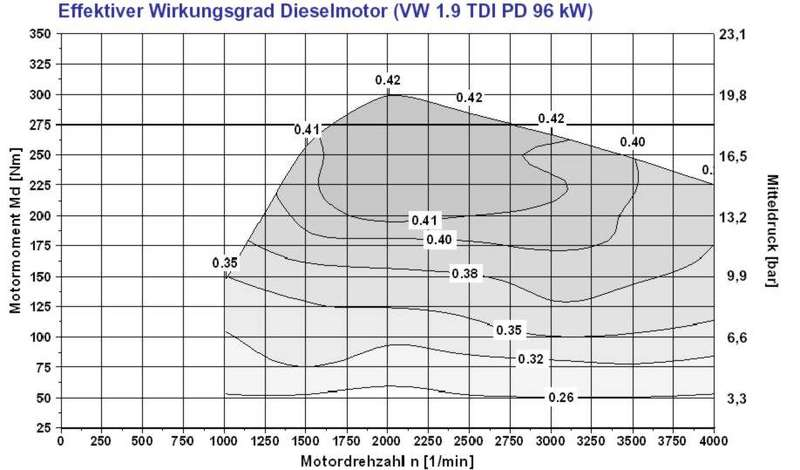
\includegraphics[width=0.8\textwidth]{images/poloMotorkennfeld}
	\caption{Motorkennfeld eines VW Polo, beachten Sie den nicht eingezeichneten Bereich \cite{SIMR.CH2-motorwirkungsgrad.SchwingungenMotorkennfeld}}\label{Fig:imgEngineVibrations}
\end{figure}

%move to the end
Gewollt war also ein möglichst wirkungsgradeffizienter Schaltvorschlag, wobei Herr Prof. Heinz Neuburger, uns diese komplexe Maschinenbau-Thematik sehr verständlich aufbereitete. Durch dieses erlangte Grundwissen war es uns  möglich, auf dieser Information für die konkrete Implementierung aufbauen zu können.
Es wurde zusammenfassend mit Prof. Neuburger festgelegt, dass ein Motor sich nicht mehr innerhalb seines optimalen  Wirkungsgrades befindet, so er 90\% seiner maximalen Drehzahl oder seines Drehmoments erreicht hat, weshalb hochgeschalten werden sollte. Außerdem wurde festgehalten, dass Motorschwingungen äußerst schädlich für Motor und Getriebe sind und deshalb bei auftretenden Schwingungen, bei niedriger Drehzahl und hoher Last, hintergeschalten werden sollte. 

Also kurz:
\begin{itemize}
	\item 90\% der max. Drehzahl oder Drehmoment --> hochschalten, wegen niedrigem Wirkungsgrad
	\item niedrige Drehzahl \&\& hohe Last --> hinunterschalten, wegen Verschleiß durch Motorschwingungen
\end{itemize}

\clearpage % DO NOT REMOVE